\documentclass{beamer}
% \usetheme{PaloAlto}
% \usetheme{Berkeley}
\usetheme{Madrid}
% \usetheme{Berlin}
%宏包
\usepackage[UTF8,noindent]{ctexcap}%避免行前缩进

%标题设置
\title{杂谈勾股定理}
\subtitle{数学史讲座之一}
\institute{九章学堂}
\author{王尔卓}
\date{\today}

%环境设置
\newtheorem{lem}{Lemma}[section]
\newtheorem{prop}{Proposition}[section]
\newtheorem{defn}{Definition}[section]
\newtheorem{coro}{Corollary}[section]
\newtheorem{theo}{Theorem}[section]
\newtheorem{exer}{Exercise}[section]
\begin{document}
% \begin{frame}
%     这是简单的一帧。

%     帧里的内容是垂直居中的。
% \end{frame}
% \begin{frame}{标题}{小标题}

%     这是简单的一帧。
% \end{frame}
\begin{frame}
    \titlepage
\end{frame}

\begin{frame}{目录}
    \tableofcontents
\end{frame}

\section{勾股定理在古代}
\begin{frame}{古中国数学}{定理发现}
    \begin{minipage}{0.5\textwidth}
    %这是一个小页面。
    \begin{figure}
    \centering
    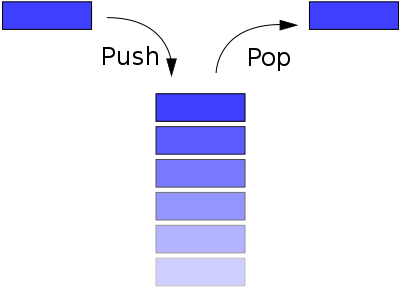
\includegraphics[width=\textwidth]{stack.png}
    \caption{栈的示例}
        \end{figure}
    \end{minipage}%
    \begin{minipage}{0.5\textwidth}
    \begin{figure}
    \centering
    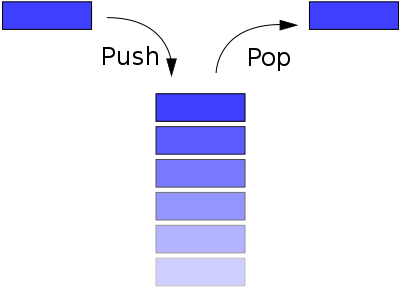
\includegraphics[width=\textwidth]{stack.png}
    \caption{XXXXX}
    \end{figure}
    \end{minipage}
\end{frame}

\begin{frame}
    \begin{theo}[Bessl恒等式]
        Bessl恒等式
    \end{theo}
    \begin{block}{勾股定理}
        \begin{equation*}
            a^2+b^2=c^2
        \end{equation*}
    \end{block}
\end{frame}

\end{document}